% =============================================================================
% FILE NAME : 01_fundamentals.tex
% DEPARTMENT: University of Tuebingen
% AUTOR     : Tom Schammo
% =============================================================================
% CONTENT   : Include for chapter "Fundamentals"
% =============================================================================


\section{RISC-V}

RISC-V \cite{riscv} is an open standard Instruction Set Architecture (ISA).
RISC-V was originally developed to support computer architecture research and education, but the authors now
aim for RISC-V to also be used in industry implementations \cite{riscv_spec}.

\subsection{ISA}

A computer program consists of several instructions.
These instructions are 'commands' that a computer understands and react to by performing certain tasks in response.
A compiler, in case of compiled languages like C, C++, Rust or Go, transforms code written by a human into instructions.
In case of interpreted languages like Python, Java or JavaScript, the code is converted into ByteCode which is then converted into
these instructions (also sometimes referred to as 'machine code') by the interpreter.
An Instruction Set is, as the name suggests, the set of instructions that a specific computer, or to be more precise,
its Central Processing Unit (CPU) can understand.
Which instructions are available depends on the hardware of a particular system.
Instruction Set Architectures abstractly describe the architecture of a computer,
like supported data types, available registers, how main memory is managed by the hardware and
which instructions  a microprocessor can execute \cite{isa}, which can then be implemented by a CPU.
ISAs are often classified by their complexity, belonging either to the set of 'complex instruction set computers' (CISC), like x86,
or 'reduced instruction set computers' (RISC) like ARM \cite{arm_architecture} or RISC-V \cite{riscv_spec}.

\subsection{RISC-V vs. ARM}

While RISC-V \cite{riscv} is an open standard ISA provided, royalty-free, by 'RISC-V International', a non-profit,
ARM \cite{arm} is developed by a company that sells licenses to other businesses that develop CPUs based on the ARM architecture.
ARM generally has a much higher market share than RISC-V due to it being used in pretty much every mobile device (phones, tablets, smartwatches)
these days, as well as many IoT devices and even laptops like the new Apple MacBooks containing the M1 system-on-a-chip (SOC).
However, NVIDIA announced its acquisition of ARM in 2020 \cite{arm_sale}, which was met with disapproval by some people.
This caused speculations, that some companies might turn to RISC-V in the future as an alternative \cite{arm_sale_speculation}.
However, the acquisition was called off in 2022 \cite{arm_sale_called_off}.


\section{Embedded AI}

With artificial intelligence (AI) becoming more and more contemporary and wide-ranging it is only consequential that is has found its way into embedded devices.
Especially with the rising trend of IoT devices and smart homes embedded AI has found its way into the hand of consumer homes.
From voice assistants like Amazon's Alexa \cite{alexa} over autonomous robots like the Roomba \cite{roomba} from iRobot to self-driving cars like Tesla's autopilot \cite{autopilot}.
However size and power requirements of those devices severely limit their capabilities, which is why the development of specialized hardware to improve performance
and power usage becomes a necessity.\\

In my thesis I'm working with the UltraTrail TC-ResNet AI Accelerator \cite{ultratrail}.
An AI Accelerator is a type of hardware accelerator specialized for artificial intelligence (AI) and machine learning (ML) applications, such as neural networks (NN).
A hardware accelerator is a set of custom-made hardware that specializes in carrying out one task only, but doing it really well.
It is created to perform solve one problem faster and/or more efficiently than a generic CPU could with the trade-off that it may not be able to do other things at all.
Examples include, but are not limited to, GPUs or, in this case, AI accelerators.\\\\


\section{Rust}

Rust \cite{rustlang} has been the language of choice for the software running on the Pulpissimo \cite{pulpissimo} that I've written for this thesis.

\subsection{Why Rust?}

While C is the industry standard for writing software for embedded systems, and C++ also being fairly popular, Rust has a couple of
advantages over those languages.\\\\
The biggest downside of C is likely the lack of memory safety, which can not only cause software to be less reliable, but
can also make a system vulnerable to different attacks, such as buffer overflows, reading uninitialized variables or use-after-free, which can compromise cybersecurity \cite{memory_safety}.\\
C++ fixes some of those issues due to the availability of smart pointers, but those are fairly 'modern' C++, thus being only available if compilers support more modern
versions of C++ (with C++ 11 starting to introduce many of concepts).
There is also no guarantee that those features have been used in any given program.
The opposite is more likely actually due to the incorporation of older software (library code written with older C++ versions in mind),
compilers not supporting new versions (especially likely with small vendors that don't have the resources to continuously update compilers for their platform),
or developers not keeping up to date with new language features and therefore not being aware of or able to use them.\\\\
Rust on the other hand can (mostly) give compile time guarantees on the software's safety and reliability.

\subsection{Memory safety and  performance}

\subsubsection{Garbage collection}

Most programming languages that try to achieve memory safety use a garbage collector to do that \cite{java_garbage_collector}.
The downside of a garbage collector however is unpredictable latency (the running program has to be stopped while the garbage collector is running) and a hit in performance.
A garbage collector first identifies pieces of memory that are no longer used \ref{fig:gc_mark}.
Then the marked pieces of memory are periodically deleted \ref{fig:gc_delete}.
After the deletion the garbage collector will 'compact' the memory to avoid memory fragmentation and improve the speed of future allocations.

\begin{figure}[htb]
    \centering
    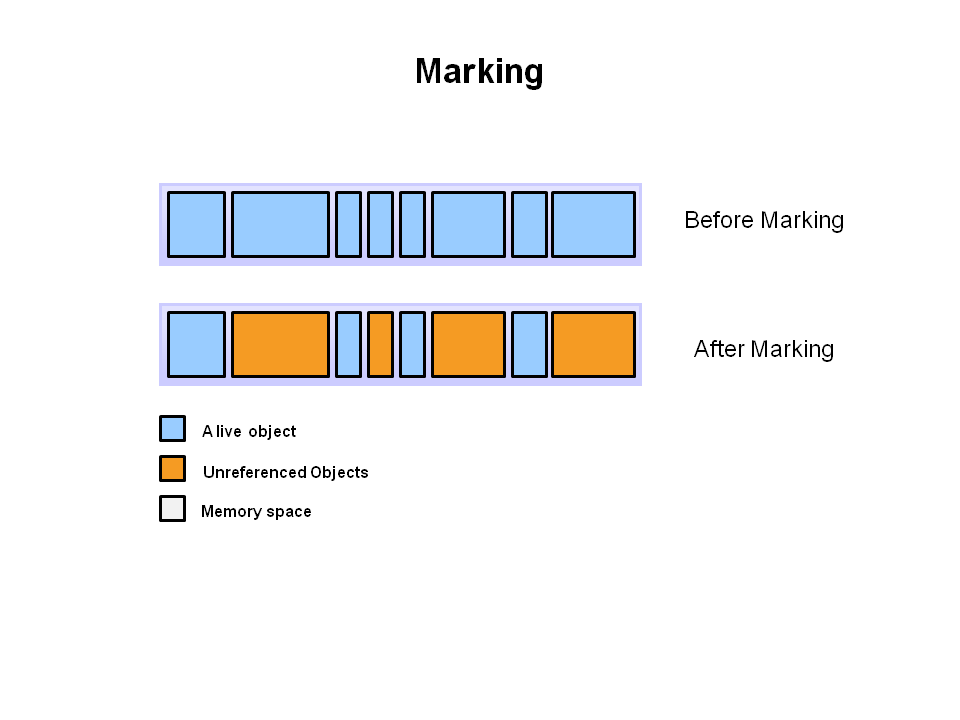
\includegraphics[width=0.9\textwidth]{figures/fundamentals_garbage_collector_marking.PNG}
    \caption[Illustration: Garbage Collector marking memory for deletion\\Source: https://www.oracle.com/webfolder/technetwork/tutorials/obe/java/gc01/images/gcslides/Slide3.png]{Garbage Collector marking memory for deletion}
    \label{fig:gc_mark}
\end{figure}

\begin{figure}[htb]
    \centering
    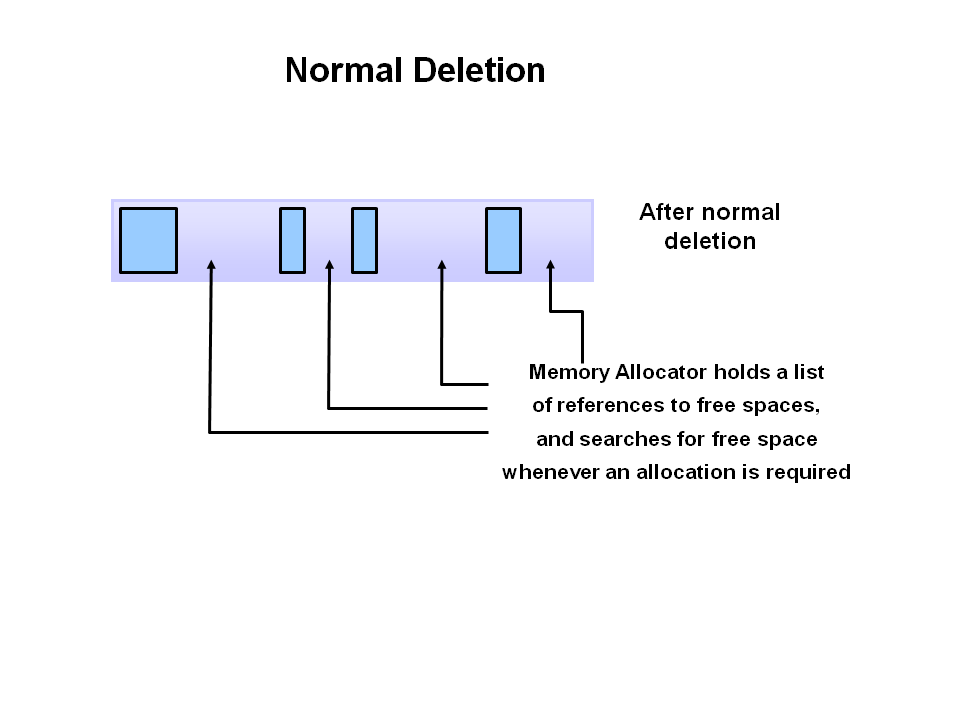
\includegraphics[width=0.9\textwidth]{figures/fundamentals_garbage_collector_deletion.PNG}
    \caption[Illustration: Garbage Collector deleting marked memory\\Source: https://www.oracle.com/webfolder/technetwork/tutorials/obe/java/gc01/images/gcslides/Slide1b.png]{Memory layout after deletion of unused pieces of memory}
    \label{fig:gc_delete}
\end{figure}

\begin{figure}[htb]
    \centering
    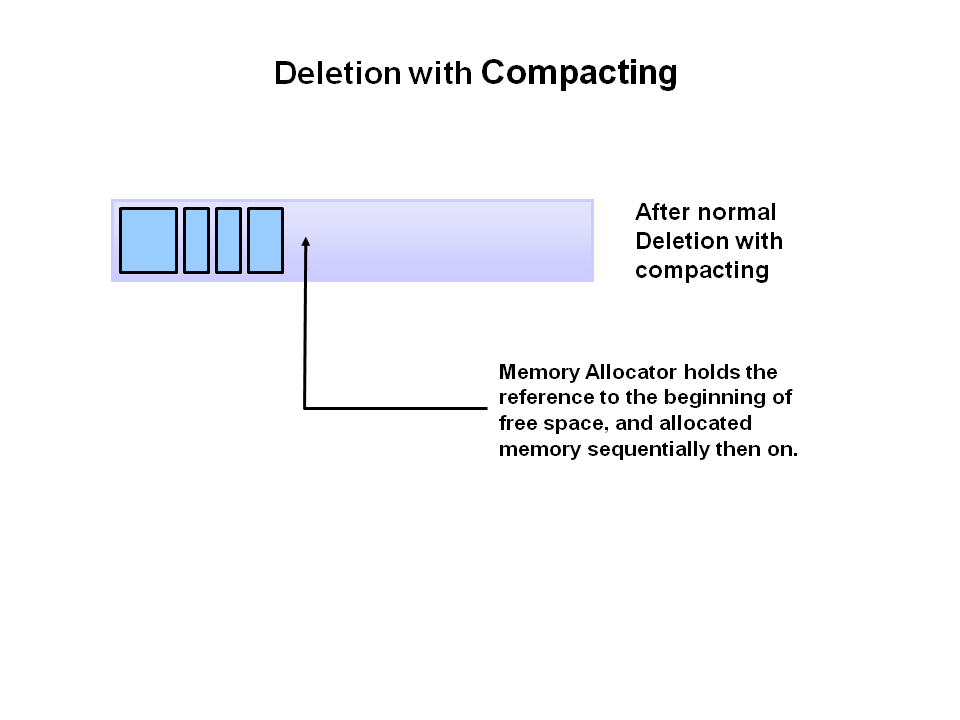
\includegraphics[width=0.9\textwidth]{figures/fundamentals_garbage_collector_compacting.PNG}
    \caption[Illustration: Garbage Collector compacting memory\\Source: https://www.oracle.com/webfolder/technetwork/tutorials/obe/java/gc01/images/gcslides/Slide4.png]{Memory layout after compacting}
    \label{fig:gc_compact}
\end{figure}

\subsubsection{Ownership in Rust}

Rust uses an 'ownership' model \cite{rust_ownership} to make memory safety guarantees at compile time and without the need of a garbage collector,
which is good for safety, and does not negatively impact performance or latency.
This model consists of 3 simple rules:
\begin{enumerate}
    \item Each value has an owner
    \item Each value can only have one owner at a time
    \item When the owner goes out of scope, the value will be dropped
\end{enumerate}

These 'owners' are generally variables. \ref{code:owner} presents a simple example of a 'value' ('\lstinline{5}') and its
'owner' ('\lstinline{owner}').\\
It doesn't matter that another 'owner' might have the same value. In the code depicted in \ref{code:two_owners}
'\lstinline{owner}' and '\lstinline{owner2}' have the same value, but they are different variables, just like in any
other programming language and have nothing to do with each other. They are different 'owners'.\\
If one variable is assigned to another, one of two things happens; if the value is saved on the stack like in
example \ref{code:copy} the value is simply copied to the second variable, and now '\lstinline{owner}' and '\lstinline{owner2}'
hold the same value, but other than that have nothing to do with each other. They are different 'owners'.\\
If the value is stored on the heap like in example \ref{code:move}, the value is not copied, because that could
be potentially very expensive.
So only the pointer (memory address), size of the data, and the capacity of the memory block is copied.
But now '\lstinline{value}' has two owners, which violates rule 2.
This rule is important because due to rule 3:
\begin{enumerate}
    \item If both variables go out of scope at the same time, the memory would be freed twice.
    \item If only one goes out of scope, the other holds the address of invalid (freed) memory.
\end{enumerate}
To avoid those things '\lstinline{value}' is considered to be 'moved' to its new owner, the variable '\lstinline{owner2}',
and the original owner ('\lstinline{owner}') is no longer valid.\\
This works similarly for functions, and these 3 rules allow the compiler to check for any mistakes that would lead to
memory issues.
However, there is one more thing that needs to be talked about; the borrow operator.
The borrow operator ('\lstinline{\&}') \cite{rust_borrow} allows other variables access to a value without changing the owner.
There follow two more rules for references and borrowing:
\begin{enumerate}
    \item There can be an infinite number of immutable references to a value.
    \item There can only be one mutable reference to a value.
\end{enumerate}
The code snippet \ref{code:borrow} displays a valid use of rule 1 and code snippet \ref{code:mut_borrow} gives both examples
of what is valid and invalid under rule 2.

\begin{lstlisting}[style=colorEX,language=Rust,caption={Simple example of a value and it's owner},label={code:owner}]
{
    let owner = 5;
}
\end{lstlisting}


\begin{lstlisting}[style=colorEX,language=Rust,caption={Simple example of a copy},label={code:copy}]
{
    let owner = 5;
    let owner2 = owner;
}
\end{lstlisting}

\begin{lstlisting}[style=colorEX,language=Rust,caption={Simple example of two owners},label={code:two_owners}]
{
    let owner = 5;
    let owner2 = 5;
}
\end{lstlisting}

\begin{lstlisting}[style=colorEX,language=Rust,caption={Simple example of a move},label={code:move}]
{
    let owner = String::from("value");
    let owner2 = owner;
}
\end{lstlisting}

\begin{lstlisting}[style=colorEX,language=Rust,caption={Simple example of a immutable borrow},label={code:borrow}]
{
    let owner = 5;
    let borrower1 = &owner;
    let borrower2 = &owner;
}
\end{lstlisting}

\begin{lstlisting}[style=colorEX,language=Rust,caption={Simple example of a mutable borrow},label={code:mut_borrow}]
{
    let owner = 5;
    let borrower = &mut owner;

    // These 2 statements are not allowed, as the value as already borrowed as mutable.
    // let borrower1 = &owner;
    // let borrower2 = &mut owner;
}
\end{lstlisting}


\subsection{Embedded Rust}

Developing software that runs directly on hardware is a bit different due to the lack of an operating system (OS).
When developing for a microcontroller (MCU) there is no OS that supervises and manages programs or facilitates communication with peripherals.
Therefore, embedded Rust programs look a little different from those that would run on a Windows, Linux or Mac computer.
\\
First, since there is no operating system to allocate memory, put the code into the right memory space and start the program.
So the developer has to take care of that when creating the executable, which is why 'special' instructions for the linker are necessary.
For Rust programs these instructions are written into a \lstinline{memory.x} file.
This file contains information about the memory layout of the hardware that the program will be running on.
An example of such a \lstinline{memory.x} file can be found in \ref{code:memory_x}.

\begin{lstlisting}[style=colorEX,caption={Example memory.x file},label={code:memory_x}]
MEMORY
{
  /* NOTE K = KiBi = 1024 bytes */
  /* RAM : ORIGIN = 0x1C000000, LENGTH = 0x0007fffc */
  RAM : ORIGIN = 0x1C000000, LENGTH = 0x00010000
  LTWO : ORIGIN = 0x1C010000, LENGTH = 0x00072000
  /* FLASH : ORIGIN = 0x1A000000, LENGTH = 8K */


}

SECTIONS
{
    .l2_data ORIGIN(LTWO) :
    {
        LONG(0x00072000);
        *(.l2_data);
    } > LTWO
}

REGION_ALIAS("FLASH", RAM);

REGION_ALIAS("REGION_TEXT", FLASH);
REGION_ALIAS("REGION_RODATA", FLASH);
REGION_ALIAS("REGION_DATA", RAM);
REGION_ALIAS("REGION_BSS", RAM);
REGION_ALIAS("REGION_HEAP", RAM);
REGION_ALIAS("REGION_STACK", RAM);

\end{lstlisting}


However, there are also quite a few differences in the actual program code. Usually Rust programs contain a main function that looks like the example in \ref{code:os_main}.
This serves as an entry for the program, and it returns nothing. After the function returns, the OS initiates its cleanup routine for the ending process like usual.

\begin{lstlisting}[style=colorEX,language=Rust,caption={Standard main function in Rust},label={code:os_main}]
fn main() {
    // contents of main function
}
\end{lstlisting}

But due to the lack of an OS, starting the program looks quite a bit differently, and is no cleanup after the program ended either.
As a matter of fact, since the program will be the only thing running on the hardware, the main function will never return, and the program
only really stops when the device is turned off.

\begin{lstlisting}[style=colorEX,language=Rust,caption={Example main function for the pulp-platform},label={code:embedded_main}]
#![no_main]

use riscv_rt::entry;

#[entry]
fn main() -> ! {
    // code
    loop {}
}
\end{lstlisting}

\ref{code:embedded_main} displays a main function alike to the ones I've used in my programs.
The '\lstinline{#![no_main]}' directive tells the compiler that I will not use the standard main function.
Since this function will never return, the return type not specify exactly that.
In Rust, return types are specified using the '\lstinline{->}', followed by the type \cite{rust_return}.
The '\lstinline{!}' indicates that the function doesn't return \cite{rust_never_type}.
\\
The '\lstinline{#[entry]}' attribute, imported by the '\lstinline{use riscv_rt::entry}' statement, is used to declare the entry point of the program \cite{riscv_rt_entry}
The requirement for this attribute is that the function never returns, which also why the loop at the end is necessary.
\\\\
This is close to a working program, but not quite there yet.
Without the OS, the device is also not able to load the standard library.
Which is why the '\lstinline{#![no_std]}' is used, as it prevents Rust from loading the standard library \cite{rust_no_std}.
However, the standard library provides a lot of useful features, like a dynamic memory allocator or a panic handler.
So these features need to be replaced by their own crates, if available.
The crates that provide those features in this case are called the '\lstinline{pulpissimo_hal}' and '\lstinline{pulpissimo_pac}'.
They act as an abstraction layer over and provide an interface to interact with the hardware.
\\
A minimal example of a running program can be found in \ref{code:min_example}.
This minimal example doesn't use any features from the '\lstinline{pulpissimo_pac}' directly, which is why it is not 'included'.
Also, the endless loop at the end is replaced by the '\lstinline{exit}' function from the '\lstinline{pulpissimo_hal}'.
This example also uses the '\lstinline{println}' macro from the '\lstinline{pulpissimo_hal}' to print messages that then can be viewed over minicom.

\begin{lstlisting}[style=colorEX,language=Rust,caption={Minimal example of a program running on the pulpissimo hardware},label={code:min_example}]
#![no_main]
#![no_std]

use riscv_rt::entry;

use panic_halt as _;
use pulpissimo_hal as hal;

use hal::{exit, println};

#[entry]
fn main() -> ! {
    println!("Hello, world!");

    exit(0)
}
\end{lstlisting}


\section{Microphone technology}

A microphone consists of a diaphragm and a transducer.
Sound waves cause the diaphragm to vibrate, and
the transducer turns those vibrations into an electrical signal.

\subsection{I2S}

The inter-IC sound ($I^2S$) \cite{i2s} bus is a serial link that has been developed especially for digital audio.
It uses three lines, one serial data line (SD), one continuous serial clock line (SCK) and one word select line (WS).
$I^2S$ can be used in different configurations, but the master always provides WS and SCK.

\subsubsection{Serial Data}

The data consists of signed integers (in two's complement).
Due to possible differences between the word lengths and neither the transmitter nor the
receiver having any knowledge about the capabilities of the other, the MSB is transmitted first.
In the transmission, the MSB has a fixed position, which means that the position of the LSB
is variable due to possible size differences between the word lengths of transmitter and receiver,
and it being dependent on the word length.\\
So when the word length of the system exceeds that of the transmitter, the LSBs are truncated
for the transmission as demonstrated in \ref{fig:truncation}.
If the receiver receives more bits than its word length, everything after the LSB
of the receiver is ignored, and if the receiver gets fewer bits than its,
the missing bits are set to 0.\\
Furthermore, data sent by the transmitter can either be synchronized with a trailing or leading edge
of the clock signal, however received data must be latched onto the leading edge.


\begin{figure}[htb]
    \centering
    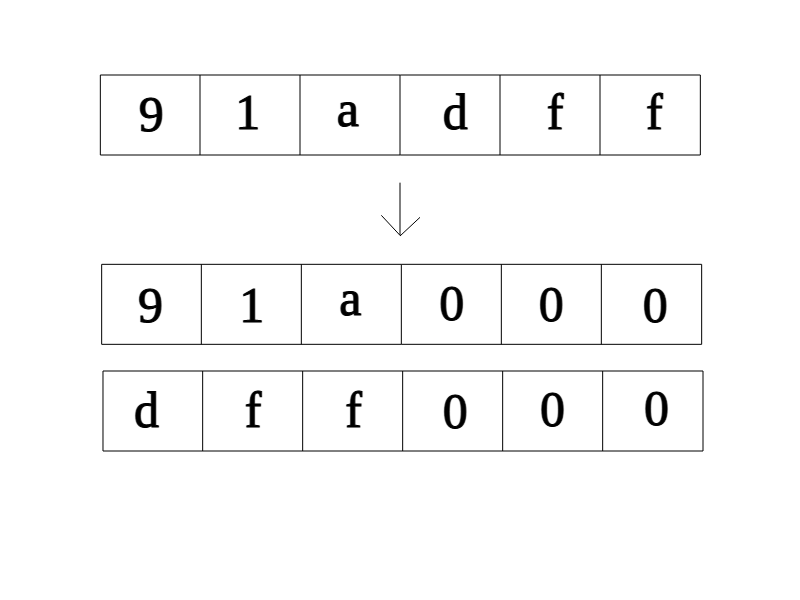
\includegraphics[width=0.9\textwidth]{figures/fundamentals_truncation.png}
    \caption[Illustration: Truncation of words]{Example of a longer word being split into two with the lower bits being set to zero}
    \label{fig:truncation}
\end{figure}

\subsubsection{Word Select}

Word select determines the transmission channel, where 0 means the left channel and 1 means the right one.
It can be changed on a trailing or leading edge of the clock signal and the WS line changes one clock period
before the MSB is transmitted.
For the purpose of what I do in this thesis, WS is not relevant and will be tied to ground unless mentioned otherwise.

\subsection{Pulse Density Modulation}

Pulse Density Modulation (PDM) is one way to represent an analog signal with a binary signal.
The density of high/low signals at a given sampling rate encodes the state of the analog signal.
So the analog signal is encoded using only 1 bit at a high sampling rate.\\
Therefore, a constant bit stream of 1s would represent that the amplitude of the analog signal is maxed out,
while a constant bit stream of 0s would represent that the amplitude of the analog signal is at its lowest value.
Alternating 1s and 0s represent an amplitude of exactly 0.\\\\
While many digital audio systems use Pule Code Modulation (PCM), which, in contrast to PDM, uses multiple bits to represent a signal,
PDM is used a lot in mobile phones \cite{pdm_utexas} due to its simplicity and low cost.
However, 1bit PCM would be much too noisy to be useful.
So to counteract the noise increase of only using 1 bit the signal is 'oversampled', thereby increasing the bandwidth of the system.
The new spectrum that is created by oversampling the signal has a frequency that is too high for the human ear.
'Noise Shaping' can then be used to 'push' noise into that new spectrum, thus removing it from the audible signal \cite{pdm_texas}.
